\subsection{Sélection de variables}
Le dernier exemple d'application que nous proposerons ici est celui de la recherche d'importance des variables. En effet, certains algorithmes de Machine Learning (comme les Random Forest), peuvent permettre de comparer l'importance des variables entre elles.

Dans la mesure où XGBoost va à l'instar des Random Forest entraîner plusieurs arbres et faire des choix sur les variables les plus pertinentes pour créer de nouvelles branches, il est possible de mettre en place un calcul d'importance des variables via XGBoost. Ce calcul peut être réalisé en utilisant par exemple le code R suivant.
\begin{lstlisting}[language=R]
bst <- xgboost(data = train$data, label = train$label, max.depth = 2, eta = 1, nthread = 2, nround = 2,objective = "binary:logistic")
importance_matrix <- xgb.importance(agaricus.train$data@Dimnames[[2]], model = bst)
xgb.plot.importance(importance_matrix)
\end{lstlisting}
Ce code permet alors d'obtenir les évaluations de la Figure~\ref{fig:feature-importance}.

\begin{figure}[h]
	\begin{margincap}
		\centering
		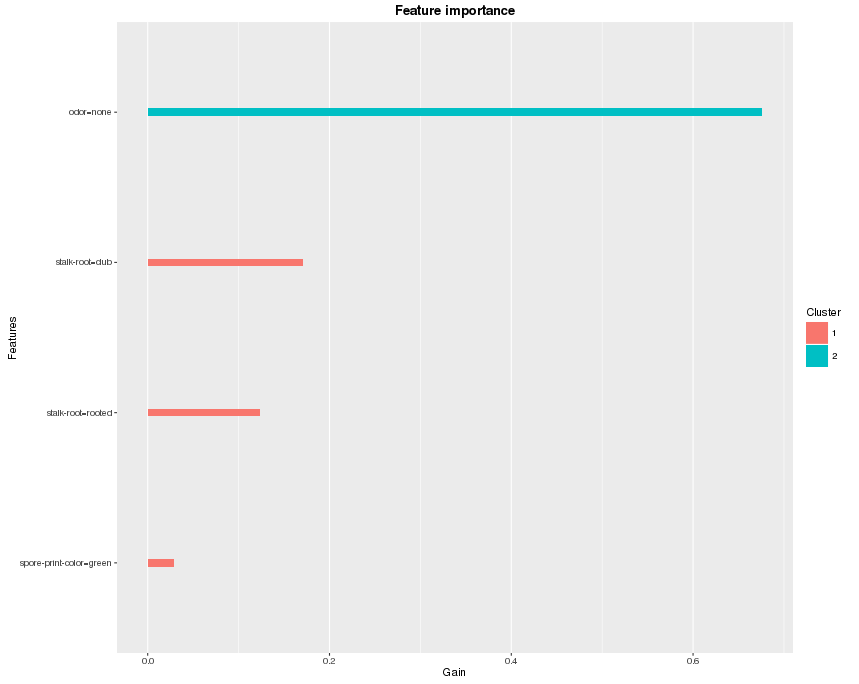
\includegraphics[width=.7\textwidth]{images/Exemples/feature-importance}
		\caption{Exemple d'affichage de l'importance des variables via XGBoost}
		\label{fig:feature-importance}
	\end{margincap}
\end{figure}

Dans ce cas particulier on remarque que la plupart de l'information est portée par le premier paramètre, les autres ne retenant qu'une part plus faible de cette dernière. En particulier, le dernier pourraît être supprimé de l'apprentissage, dans la mesure où il semble peu révélateur.
